\section{Flujo de trabajo en GIT}
\frame
{
\frametitle{Flujo de trabajo en GIT}
\begin{center}
 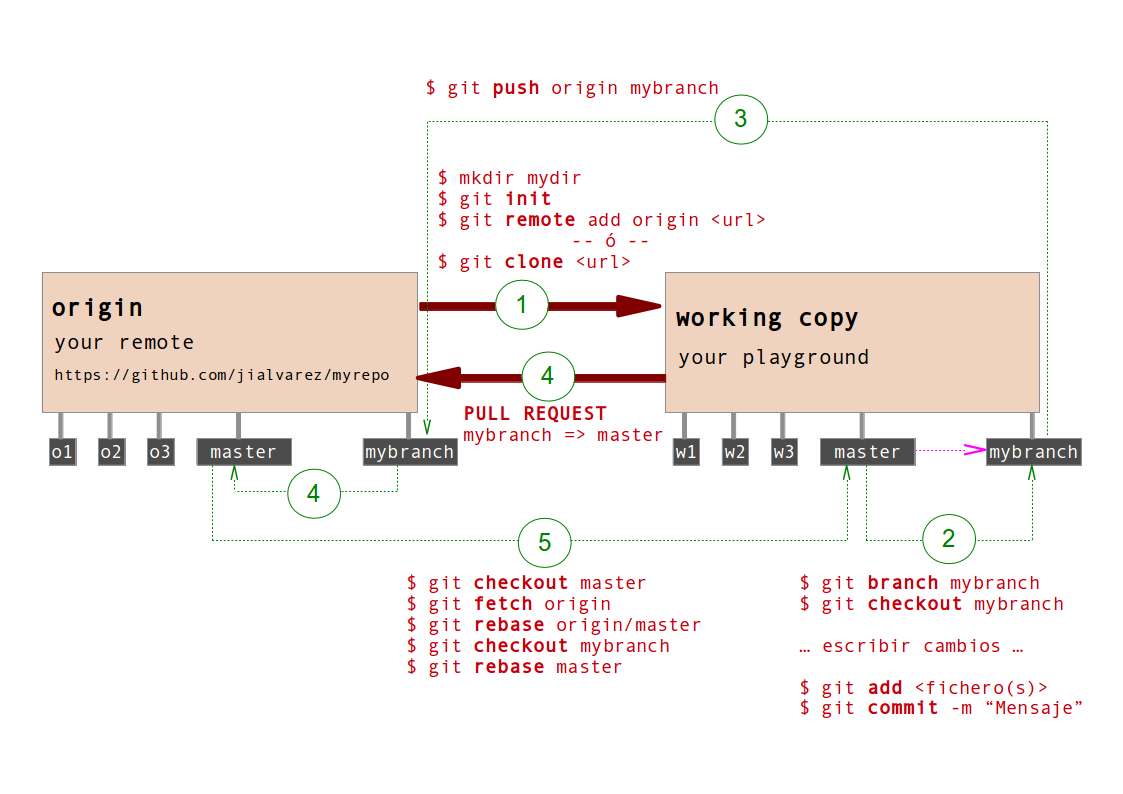
\includegraphics[height=7cm]{imgs/gitworkflow.png}
\end{center}
}

\frame
{
\frametitle{Punteros: HEAD, origin...}
}

\frame
{
\frametitle{Etapas de un fichero (I)}
\begin{framed}
\# \textbf{Archivos sin seguimiento:}\\
\#   (use git add <archivo>... para incluir lo que se ha de ejecutar)\\
\#\\
\#	\textcolor{red}{fichero.tex}
\end{framed}

\begin{itemize}
 \item Son archivos que aún no forman parte del repositorio local ni del remoto
 \item Al añadirlos pasan a la etapa III
\end{itemize}
}

\frame
{
\frametitle{Etapas de un fichero (II)}
\begin{framed}
\# \textbf{Cambios no preparados para el commit:}\\
\#   (use git add <archivo>... para actualizar lo que se ejecutará)\\
\#   (use git checkout -{}- <archivo>... para descartar cambios en el directorio de trabajo)\\
\#\\
\#	\textcolor{red}{modificado:   advanced.tex}\\
\#	\textcolor{red}{modificado:   principal.pdf}\\
\end{framed}

\begin{itemize}
 \item Son ficheros ya añadidos previamente pero que aún no han sido \textit{marcados} para comitear
 \item Al añadirlos pasan a la etapa III
 \item Si le aplicamos un \textit{checkout} vuelven a la etapa I
\end{itemize}
}

\frame
{
\frametitle{Etapas de un fichero (III)}
\begin{framed}
\# \textbf{Cambios para hacer commit:}\\
\#   (use git reset HEAD <archivo>...para eliminar stage)\\
\#\\
\#	\textcolor{green}{modificado:   workflow.tex}\\
\end{framed}

\begin{itemize}
 \item Son ficheros ya añadidos previamente y marcados para comitear
 \item Si le aplicamos un \textit{reset HEAD} vuelven a la etapa II
 \item En esta etapa es donde se puede \textit{\textbf{comitear}} y hacer \textit{\textbf{push}}
\end{itemize}
}

\frame
{
\frametitle{Git branching}

\begin{tabular}[t]{m{5cm}m{6cm}}
   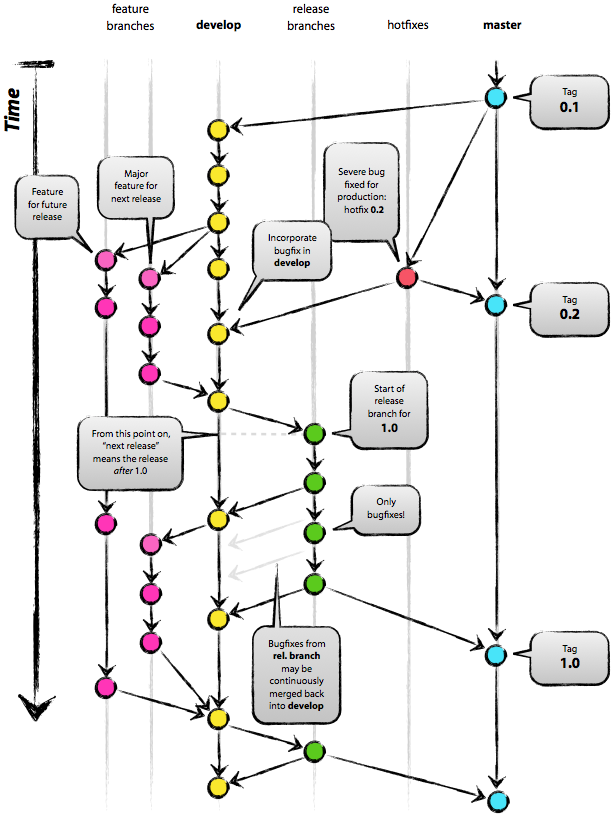
\includegraphics[height=8cm]{imgs/gitbranching.png} 
   &
   \begin{itemize}
    \addtolength{\itemindent}{0.4cm}
    \item Reglas propuestas por Vincent Driessen
    \item Ramas \textbf{master} (commits producción) y \textbf{develop} (siguiente versión planificada)
    \item Ramas \textbf{feature} (funcionalidad concreta). Se originan a partir de \textbf{develop} y vuelven a \textbf{develop}
    \item Ramas \textbf{release} (siguiente versión en producción). Se originan de \textbf{develop} y pasan a master o \textbf{develop}.
    \item Ramas \textbf{hotfix} (bugs en producción). Se originan a partir de \textbf{master} y vuelven a \textbf{master} o \textbf{develop}.
   \end{itemize}
\end{tabular}
}